\section{INTRODUCTION}

\IEEEPARstart{F}{or} Proj.2, we implement a CNN accelerating architecture based on \textit{Optimizing the Convolution Operation to Accelerate Deep Neural Networks}\cite{maOptimizingConvolutionOperation2018}.

The research question of the paper relies on the fact that prior works lack fully studying the convolution loop optimization before the hardware design phase, resulting in accelerator which hardly exploit the data reuse and manage data movement efficiently. So the author of this paper studies CNN-related techniques, e.g. loop unrolling, tiling and interchange, by quantitatively analyzing and optimizing the design objectives of the CNN accelerator based on multiple design variables. At the same time, based on conclusions above, the author proposed a hardware CNN accelerator which concerns:

\begin{itemize}
    \item limited computational resources
    \item storage capacity
    \item off-chip communication
\end{itemize}
providing simultaneous maximization of resource utilization and data reuse, and minimization of data communication.

The reason we choose this paper is that, it provides not only a smart new design, but presents a very detailed and in-depth analysis of the basis of convolution loop optimization as well, making it a perfect choice for us to study.

Below is the scheme proposed:

\begin{figure}[!htb]
    \centering
    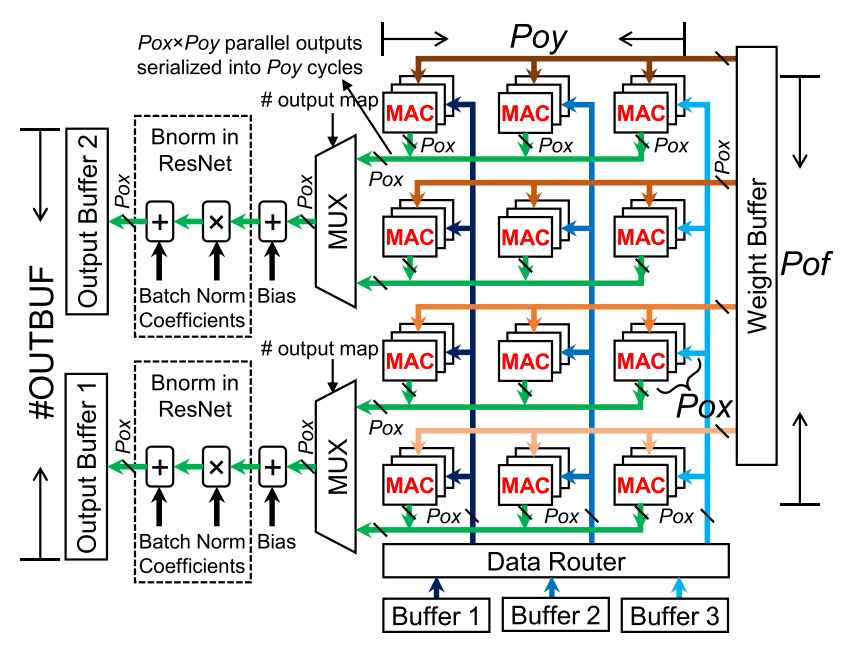
\includegraphics[width=0.9\columnwidth]{../figures/Arch.png}
    \caption{Convolution acceleration architecture with Pox × Poy × Pof MAC units.}
    \label{fig:Arch}
\end{figure}

During the process of our reproduction, we encounter some difficulties and also discover some flaws that should be corrected or could be further optimized.